\RequirePackage{atbegshi} % Background stuff below trim marks
\AtBeginShipoutInit
\documentclass[avery5371]{flashcards}

%%% PACKAGES
\usepackage{xkeyval}% kvp
\usepackage{changepage} % page check
\strictpagecheck
\usepackage{amssymb} % boxes
\usepackage{amsmath} % maths
\usepackage{lipsum} % dummy text
\usepackage{ragged2e} % switch commands to flushLeft/right
\usepackage{graphicx} % include jged, png, etc.
\graphicspath{{./images/}} 
\usepackage[export]{adjustbox} % use adjustbox keys in includegraphics, e.g. max height/width
\usepackage{svg} % include svg using inkscape
\usepackage[top]{background} % Background stuff
\usepackage{eso-pic}
\usepackage{tikz} % tikz drawing
\usepackage{xcolor} % custom colors
\definecolor{uniscielblue}{RGB}{4,146,191}
\definecolor{uniscielpink}{RGB}{231,33,90}
\definecolor{uniscielgrey}{RGB}{103,104,104}
\definecolor{physicsviolet}{RGB}{70,51,116}
% Blue : #0492bf
% Pink : #e7215a
% Grey : #676868
% Violet : #463374

%%% FONTS %%%%
\usepackage[no-math]{fontspec}
\setsansfont{Dancing Script}
\setmainfont{Roboto Condensed}

%%% GEOMETRY AND BLEED MARKS %%%
\geometry{
    papersize = {200 truemm, 297 truemm},
    margin = 0 truemm,
    % marginparwidth = 0 truemm,
    % marginparsep = 0 truemm
}

\usepackage[
width = 200 truemm,
height =  297 truemm,
noinfo,
center
]{crop}    

%%% FLASHCARDS PARAMETERS %%%
% Card size and margins
\renewcommand{\cardpapermode}{portrait}
\renewcommand{\cardrows}{3}
\renewcommand{\cardcolumns}{2}
\setlength{\cardwidth}{10 cm}
\setlength{\cardheight}{8 cm}
\setlength{\cardmargin}{3 mm}
\setlength{\topoffset}{0 mm}
\setlength{\oddoffset}{0 mm}
\setlength{\evenoffset}{0 mm}

% Card Background
\SetBgScale{1.0}                          % Select scale factor
\SetBgAngle{0.0}                          % Select rotation
% \SetBgOpacity{0.5}                        % Select opacity
% \SetBgContents{\bgimage{0.15}{0.8}}       % Set tikz picture
% \SetBgPosition{current page.north west}   % Select location

% Card styles and fonts
\cardfrontstyle[\footnotesize]{plain}
\cardbackstyle[\footnotesize]{plain}

%%% CUSTOM COMMANDS %%%
% KVP
\makeatletter

\define@cmdkey{One}[FCone@]{complexityLevel}{}
\define@cmdkey{One}[FCone@]{subject}{}
\define@cmdkey{One}[FCone@]{theme}{}
\define@cmdkey{One}[FCone@]{qrcode}{}

\define@cmdkey{Two}[FCtwo@]{complexityLevel}{}
\define@cmdkey{Two}[FCtwo@]{subject}{}
\define@cmdkey{Two}[FCtwo@]{theme}{}
\define@cmdkey{Two}[FCtwo@]{qrcode}{}

\define@cmdkey{Three}[FCthree@]{complexityLevel}{}
\define@cmdkey{Three}[FCthree@]{subject}{}
\define@cmdkey{Three}[FCthree@]{theme}{}
\define@cmdkey{Three}[FCthree@]{qrcode}{}

\define@cmdkey{Four}[FCfour@]{complexityLevel}{}
\define@cmdkey{Four}[FCfour@]{subject}{}
\define@cmdkey{Four}[FCfour@]{theme}{}
\define@cmdkey{Four}[FCfour@]{qrcode}{}

\define@cmdkey{Five}[FCfive@]{complexityLevel}{}
\define@cmdkey{Five}[FCfive@]{subject}{}
\define@cmdkey{Five}[FCfive@]{theme}{}
\define@cmdkey{Five}[FCfive@]{qrcode}{}

\define@cmdkey{Six}[FCsix@]{complexityLevel}{}
\define@cmdkey{Six}[FCsix@]{subject}{}
\define@cmdkey{Six}[FCsix@]{theme}{}
\define@cmdkey{Six}[FCsix@]{qrcode}{}

\presetkeys{Two}{
    complexityLevel = none,
    subject = none,
    theme = none,
    qrcode = none
}{}
\presetkeys{Three}{
    complexityLevel = none,
    subject = none,
    theme = none,
    qrcode = none
}{}
\presetkeys{Four}{
    complexityLevel = none,
    subject = none,
    theme = none,
    qrcode = none
}{}
\presetkeys{Five}{
    complexityLevel = none,
    subject = none,
    theme = none,
    qrcode = none
}{}
\presetkeys{Six}{
    complexityLevel = none,
    subject = none,
    theme = none,
    qrcode = none
}{}
    
\newcommand{\cardbackground}[1]{
    \SetBgContents{
        \AddToShipoutPictureBG*{
            \begin{tikzpicture}[remember picture, overlay]
                % Front + 8.1 cm
                % Back + 8.1 cm
                \checkoddpage
                \ifoddpage
                %%%%%% FC ONE
                \ifnum#1>0
                    % Subject front header
                    \node at ([xshift = 4 cm, yshift = -1.13 cm]current page.north west) {
                        \includesvg[width = 0.8\cardwidth]{\frontheader}
                    };
                    % Subject front footer
                    \node at ([xshift = 6 cm, yshift = -7.45 cm]current page.north west) {
                        \includesvg[width = 0.8\cardwidth]{\frontfooter}
                    };
                    % Subject icon
                    \node [opacity = 1] at ([xshift = 1 cm, yshift = -1.1 cm]current page.north west) {
                        \includesvg[height = 0.160\cardheight]{icons/\subjecticon}
                    };
                    % Subject text
                    \node [opacity = 1] at ([xshift = 3 cm, yshift = -0.85 cm]current page.north west) {
                        \color{white}
                        \Large
                        \textsf{\FCone@subject}
                    };
                    % Theme
                    \node [opacity = 1] at ([xshift = 7 cm, yshift = -2.1 cm]current page.north west) {
                        \begin{varwidth}{0.5\cardwidth}
                            \setlength{\parskip}{0 cm}
                            \color{uniscielblue}
                            \RaggedLeft
                            \large
                            \textsf{\FCone@theme}
                        \end{varwidth}
                    };
                    % University front logo
                    \node [opacity=1] at ([xshift = 8.25 cm, yshift = -7.45 cm]current page.north west) {                    
                        \includegraphics[max height = 0.125\cardheight, center, keepaspectratio]{\frontuniversitylogo}
                    };
                    % Complexity level
                    \node [opacity=1] at ([xshift = 2.5 cm, yshift = -7.05 cm]current page.north west) {
                        \color{uniscielpink}
                        \textsf{\textit{\FCone@complexityLevel}}
                    };
                \fi
                %%%%%% FC TWO
                \ifnum #1>1
                % Subject front header
                    \node at ([xshift = 14 cm, yshift = -1.13 cm]current page.north west) {
                        \includesvg[width = 0.8\cardwidth]{\frontheader}
                    };
                    % Subject front footer
                    \node at ([xshift = 16 cm, yshift = -7.45 cm]current page.north west) {
                        \includesvg[width = 0.8\cardwidth]{\frontfooter}
                    };
                    % Subject icon
                    \node [opacity = 1] at ([xshift = 11 cm, yshift = -1.1 cm]current page.north west) {
                        \includesvg[height = 0.160\cardheight]{icons/\subjecticon}
                    };
                    % Subject text
                    \node [opacity = 1] at ([xshift = 13 cm, yshift = -0.85 cm]current page.north west) {
                        \color{white}
                        \Large
                        \textsf{\FCtwo@subject}
                    };
                    % Theme
                    \node [opacity = 1] at ([xshift = 17 cm, yshift = -2.1 cm]current page.north west) {
                        \begin{varwidth}{0.5\cardwidth}
                            \setlength{\parskip}{0 cm}
                            \color{uniscielblue}
                            \RaggedLeft
                            \large
                            \textsf{\FCtwo@theme}
                        \end{varwidth}
                    };
                    % University front logo
                    \node [opacity=1] at ([xshift = 18.25 cm, yshift = -7.45 cm]current page.north west) {                    
                        \includegraphics[max height = 0.125\cardheight, center, keepaspectratio]{\frontuniversitylogo}
                    };
                    % Complexity level
                    \node [opacity=1] at ([xshift = 12.5 cm, yshift = -7.05 cm]current page.north west) {
                        \color{uniscielpink}
                        \textsf{\textit{\FCtwo@complexityLevel}}
                    };
                \fi
                %%%%%% FC THREE
                \ifnum #1>2
                    % Subject front header
                    \node at ([xshift = 4 cm, yshift = -9.23 cm]current page.north west) {
                        \includesvg[width = 0.8\cardwidth]{\frontheader}
                    };
                    % Subject front footer
                    \node at ([xshift = 6 cm, yshift = -15.55 cm]current page.north west) {
                        \includesvg[width = 0.8\cardwidth]{\frontfooter}
                    };
                    % Subject icon
                    \node [opacity = 1] at ([xshift = 1 cm, yshift = -9.2 cm]current page.north west) {
                        \includesvg[height = 0.160\cardheight]{icons/\subjecticon}
                    };
                    % Subject text
                    \node [opacity = 1] at ([xshift = 3 cm, yshift = -8.95 cm]current page.north west) {
                        \color{white}
                        \Large
                        \textsf{\FCthree@subject}
                    };
                    % Theme
                    \node [opacity = 1] at ([xshift = 7 cm, yshift = -10.2 cm]current page.north west) {
                        \begin{varwidth}{0.5\cardwidth}
                            \setlength{\parskip}{0 cm}
                            \color{uniscielblue}
                            \RaggedLeft
                            \large
                            \textsf{\FCthree@theme}
                        \end{varwidth}
                    };
                    % University front logo
                    \node [opacity=1] at ([xshift = 8.25 cm, yshift = -15.45 cm]current page.north west) {                    
                        \includegraphics[max height = 0.125\cardheight, center, keepaspectratio]{\frontuniversitylogo}
                    };
                    % Complexity level
                    \node [opacity=1] at ([xshift = 2.5 cm, yshift = -15.15 cm]current page.north west) {
                        \color{uniscielpink}
                        \textsf{\textit{\FCthree@complexityLevel}}
                    };
                \fi
                %%%%%% FC FOUR
                \ifnum #1>3
                    % Subject front header
                    \node at ([xshift = 14 cm, yshift = -9.23 cm]current page.north west) {
                        \includesvg[width = 0.8\cardwidth]{\frontheader}
                    };
                    % Subject front footer
                    \node at ([xshift = 16 cm, yshift = -15.55 cm]current page.north west) {
                        \includesvg[width = 0.8\cardwidth]{\frontfooter}
                    };
                    % Subject icon
                    \node [opacity = 1] at ([xshift = 11 cm, yshift = -9.2 cm]current page.north west) {
                        \includesvg[height = 0.160\cardheight]{icons/\subjecticon}
                    };
                    % Subject text
                    \node [opacity = 1] at ([xshift = 13 cm, yshift = -8.95 cm]current page.north west) {
                        \color{white}
                        \Large
                        \textsf{\FCfour@subject}
                    };
                    % Theme
                    \node [opacity = 1] at ([xshift = 17 cm, yshift = -10.2 cm]current page.north west) {
                        \begin{varwidth}{0.5\cardwidth}
                            \setlength{\parskip}{0 cm}
                            \color{uniscielblue}
                            \RaggedLeft
                            \large
                            \textsf{\FCfour@theme}
                        \end{varwidth}
                    };
                    % University front logo
                    \node [opacity=1] at ([xshift = 18.25 cm, yshift = -15.45 cm]current page.north west) {                    
                        \includegraphics[max height = 0.125\cardheight, center, keepaspectratio]{\frontuniversitylogo}
                    };
                    % Complexity level
                    \node [opacity=1] at ([xshift = 12.5 cm, yshift = -15.15 cm]current page.north west) {
                        \color{uniscielpink}
                        \textsf{\textit{\FCfour@complexityLevel}}
                    };
                \fi
                %%%%%% FC FIVE
                \ifnum #1>4
                    % Subject front header
                    \node at ([xshift = 4 cm, yshift = -17.33 cm]current page.north west) {
                        \includesvg[width = 0.8\cardwidth]{\frontheader}
                    };
                    % Subject front footer
                    \node at ([xshift = 6 cm, yshift = -23.65 cm]current page.north west) {
                        \includesvg[width = 0.8\cardwidth]{\frontfooter}
                    };
                    % Subject icon
                    \node [opacity = 1] at ([xshift = 1 cm, yshift = -17.3 cm]current page.north west) {
                        \includesvg[height = 0.160\cardheight]{icons/\subjecticon}
                    };
                    % Subject text
                    \node [opacity = 1] at ([xshift = 3 cm, yshift = -17.05 cm]current page.north west) {
                        \color{white}
                        \Large
                        \textsf{\FCfive@subject}
                    };
                    % Theme
                    \node [opacity = 1] at ([xshift = 7 cm, yshift = -18.3 cm]current page.north west) {
                        \begin{varwidth}{0.5\cardwidth}
                            \setlength{\parskip}{0 cm}
                            \color{uniscielblue}
                            \RaggedLeft
                            \large
                            \textsf{\FCfive@theme}
                        \end{varwidth}
                    };
                    % University front logo
                    \node [opacity=1] at ([xshift = 8.25 cm, yshift = -23.55 cm]current page.north west) {
                        \includegraphics[max height = 0.125\cardheight, center, keepaspectratio]{\frontuniversitylogo}
                    };
                    % Complexity level
                    \node [opacity=1] at ([xshift = 2.5 cm, yshift = -23.25 cm]current page.north west) {
                        \color{uniscielpink}
                        \textsf{\textit{\FCfive@complexityLevel}}
                    };
                \fi
                %%%%%% FC SIX
                \ifnum #1>5
                    % Subject front header
                    \node at ([xshift = 14 cm, yshift = -17.33 cm]current page.north west) {
                        \includesvg[width = 0.8\cardwidth]{\frontheader}
                    };
                    % Subject front footer
                    \node at ([xshift = 16 cm, yshift = -23.65 cm]current page.north west) {
                        \includesvg[width = 0.8\cardwidth]{\frontfooter}
                    };
                    % Subject icon
                    \node [opacity = 1] at ([xshift = 11 cm, yshift = -17.3 cm]current page.north west) {
                        \includesvg[height = 0.160\cardheight]{icons/\subjecticon}
                    };
                    % Subject text
                    \node [opacity = 1] at ([xshift = 13 cm, yshift = -17.05 cm]current page.north west) {
                        \color{white}
                        \Large
                        \textsf{\FCsix@subject}
                    };
                    % Theme
                    \node [opacity = 1] at ([xshift = 17 cm, yshift = -18.3 cm]current page.north west) {
                        \begin{varwidth}{0.5\cardwidth}
                            \setlength{\parskip}{0 cm}
                            \color{uniscielblue}
                            \RaggedLeft
                            \large
                            \textsf{\FCsix@theme}
                        \end{varwidth}
                    };
                    % University front logo
                    \node [opacity=1] at ([xshift = 18.25 cm, yshift = -23.55 cm]current page.north west) {                    
                        \includegraphics[max height = 0.125\cardheight, center, keepaspectratio]{\frontuniversitylogo}
                    };
                    % Complexity level
                    \node [opacity=1] at ([xshift = 12.5 cm, yshift = -23.25 cm]current page.north west) {
                        \color{uniscielpink}
                        \textsf{\textit{\FCsix@complexityLevel}}
                    };
                \fi
                \else
                %%%%%% FC ONE
                \ifnum #1>0
                    % Back background
                    \node at ([xshift = 15 cm, yshift = -4.1 cm]current page.north west) {
                        \includesvg[width = 1\cardwidth]{\backbackground}
                    };
                    % Subject back header
                    \node at ([xshift = 14 cm, yshift = -1.13 cm]current page.north west) {
                        \includesvg[width = 0.8\cardwidth]{\backheader}
                    };
                    % Subject back footer
                    \node at ([xshift = 16 cm, yshift = -7.5 cm]current page.north west) {
                        \includesvg[width = 0.8\cardwidth]{\backfooter}
                    };
                    % QR Code
                    \node at ([xshift = 11 cm, yshift = -1.1 cm]current page.north west) {
                        \includegraphics[width = 0.120\cardwidth, keepaspectratio]{\FCone@qrcode}
                    };
                    % Subject text
                    \node [opacity = 1] at ([xshift = 13 cm, yshift = -0.85 cm]current page.north west) {
                        \color{physicsviolet}
                        \Large
                        \textsf{\FCone@subject}
                    };
                    % University back logo
                    \node [opacity=1] at ([xshift = 18.25 cm, yshift = -7.5 cm]current page.north west) {
                        \includesvg[height = 0.110\cardheight]{\backuniversitylogo}
                    };
                \fi
                %%%%%% FC TWO
                \ifnum #1>1
                    % Back background
                    \node at ([xshift = 5 cm, yshift = -4.1 cm]current page.north west) {
                        \includesvg[width = 1\cardwidth]{\backbackground}
                    };
                    % Subject back header
                    \node at ([xshift = 4 cm, yshift = -1.13 cm]current page.north west) {
                        \includesvg[width = 0.8\cardwidth]{\backheader}
                    };
                    % Subject back footer
                    \node at ([xshift = 6 cm, yshift = -7.5 cm]current page.north west) {
                        \includesvg[width = 0.8\cardwidth]{\backfooter}
                    };
                    % QR Code
                    \node at ([xshift = 1 cm, yshift = -1.1 cm]current page.north west) {
                        \includegraphics[width = 0.120\cardwidth, keepaspectratio]{\FCtwo@qrcode}
                    };
                    % Subject text
                    \node [opacity = 1] at ([xshift = 3 cm, yshift = -0.85 cm]current page.north west) {
                        \color{physicsviolet}
                        \Large
                        \textsf{\FCtwo@subject}
                    };
                    % University back logo
                    \node [opacity=1] at ([xshift = 8.25 cm, yshift = -7.5 cm]current page.north west) {
                        \includesvg[height = 0.110\cardheight]{\backuniversitylogo}
                    };
                \fi
                %%%%%% FC THREE
                \ifnum #1>2
                    % Back background
                    \node at ([xshift = 15 cm, yshift = -12.2 cm]current page.north west) {
                        \includesvg[width = 1\cardwidth]{\backbackground}
                    };
                    % Subject back header
                    \node at ([xshift = 14 cm, yshift = -9.23 cm]current page.north west) {
                        \includesvg[width = 0.8\cardwidth]{\backheader}
                    };
                    % Subject back footer
                    \node at ([xshift = 16 cm, yshift = -15.6 cm]current page.north west) {
                        \includesvg[width = 0.8\cardwidth]{\backfooter}
                    };
                    % QR Code
                    \node at ([xshift = 11 cm, yshift = -9.2 cm]current page.north west) {
                        \includegraphics[width = 0.120\cardwidth, keepaspectratio]{\FCthree@qrcode}
                    };
                    % Subject text
                    \node [opacity = 1] at ([xshift = 13 cm, yshift = -8.95 cm]current page.north west) {
                        \color{physicsviolet}
                        \Large
                        \textsf{\FCthree@subject}
                    };
                    % University back logo
                    \node [opacity=1] at ([xshift = 18.25 cm, yshift = -15.6 cm]current page.north west) {
                        \includesvg[height = 0.110\cardheight]{\backuniversitylogo}
                    };
                \fi
                %%%%%% FC FOUR
                \ifnum #1>3
                    % Back background
                    \node at ([xshift = 5 cm, yshift = -12.2 cm]current page.north west) {
                        \includesvg[width = 1\cardwidth]{\backbackground}
                    };
                    % Subject back header
                    \node at ([xshift = 4 cm, yshift = -9.23 cm]current page.north west) {
                        \includesvg[width = 0.8\cardwidth]{\backheader}
                    };
                    % Subject back footer
                    \node at ([xshift = 6 cm, yshift = -15.6 cm]current page.north west) {
                        \includesvg[width = 0.8\cardwidth]{\backfooter}
                    };
                    % QR Code
                    \node at ([xshift = 1 cm, yshift = -9.2 cm]current page.north west) {
                        \includegraphics[width = 0.120\cardwidth, keepaspectratio]{\FCfour@qrcode}
                    };
                    % Subject text
                    \node [opacity = 1] at ([xshift = 3 cm, yshift = -8.95 cm]current page.north west) {
                        \color{physicsviolet}
                        \Large
                        \textsf{\FCfour@subject}
                    };
                    % University back logo
                    \node [opacity=1] at ([xshift = 8.25 cm, yshift = -15.6 cm]current page.north west) {
                        \includesvg[height = 0.110\cardheight]{\backuniversitylogo}
                    };
                \fi
                %%%%%% FC FIVE
                \ifnum #1>4
                    % Back background
                    \node at ([xshift = 15 cm, yshift = -20.3 cm]current page.north west) {
                        \includesvg[width = 1\cardwidth]{\backbackground}
                    };
                    % Subject back header
                    \node at ([xshift = 14 cm, yshift = -17.33 cm]current page.north west) {
                        \includesvg[width = 0.8\cardwidth]{\backheader}
                    };
                    % Subject back footer
                    \node at ([xshift = 16 cm, yshift = -23.7 cm]current page.north west) {
                        \includesvg[width = 0.8\cardwidth]{\backfooter}
                    };
                    % QR Code
                    \node at ([xshift = 11 cm, yshift = -17.3 cm]current page.north west) {
                        \includegraphics[width = 0.120\cardwidth, keepaspectratio]{\FCfive@qrcode}
                    };
                    % Subject text
                    \node [opacity = 1] at ([xshift = 13 cm, yshift = -17.05 cm]current page.north west) {
                        \color{physicsviolet}
                        \Large
                        \textsf{\FCfive@subject}
                    };
                    % University back logo
                    \node [opacity=1] at ([xshift = 18.25 cm, yshift = -23.7 cm]current page.north west) {
                        \includesvg[height = 0.110\cardheight]{\backuniversitylogo}
                    };
                \fi
                %%%%%% FC SIX
                \ifnum #1>5
                    % Back background
                    \node at ([xshift = 5 cm, yshift = -20.3 cm]current page.north west) {
                        \includesvg[width = 1\cardwidth]{\backbackground}
                    };
                    % Subject back header
                    \node at ([xshift = 4 cm, yshift = -17.33 cm]current page.north west) {
                        \includesvg[width = 0.8\cardwidth]{\backheader}
                    };
                    % Subject back footer
                    \node at ([xshift = 6 cm, yshift = -23.7 cm]current page.north west) {
                        \includesvg[width = 0.8\cardwidth]{\backfooter}
                    };
                    % QR Code
                    \node at ([xshift = 1 cm, yshift = -17.3 cm]current page.north west) {
                        \includegraphics[width = 0.120\cardwidth, keepaspectratio]{\FCsix@qrcode}
                    };
                    % Subject text
                    \node [opacity = 1] at ([xshift = 3 cm, yshift = -17.05 cm]current page.north west) {
                        \color{physicsviolet}
                        \Large
                        \textsf{\FCsix@subject}
                    };
                    % University back logo
                    \node [opacity=1] at ([xshift = 8.25 cm, yshift = -23.7 cm]current page.north west) {
                        \includesvg[height = 0.110\cardheight]{\backuniversitylogo}
                    };
                \fi
                \fi
            \end{tikzpicture}
        }           
    }
}
\makeatother
\newcommand{\backgroundparam}[8]{
    \providecommand{\subjecticon}{#1}
    \providecommand{\frontheader}{#2}
    \providecommand{\frontfooter}{#3}
    \providecommand{\backbackground}{#4}
    \providecommand{\backheader}{#5}
    \providecommand{\backfooter}{#6}
    \providecommand{\frontuniversitylogo}{#7}
    \providecommand{\backuniversitylogo}{#8}
    \renewcommand{\subjecticon}{#1}
    \renewcommand{\frontheader}{#2}
    \renewcommand{\frontfooter}{#3}
    \renewcommand{\backbackground}{#4}
    \renewcommand{\backheader}{#5}
    \renewcommand{\backfooter}{#6}
    \renewcommand{\frontuniversitylogo}{#7}
    \renewcommand{\backuniversitylogo}{#8}
}


\begin{document}

\backgroundparam
{physique} % subject icon
{physique-precropped-front-header}% Front header filename
{physique-precropped-front-footer}% Front footer filename
{physique-precropped-back-background}% Back background filename
{physique-precropped-back-header}% Back header filename
{physique-precropped-back-footer}% Back footer filename
{front_university_logo}% Front university logo
{back_university_logo}% Back university logo

% For 6 flashcards
\setkeys{One}{
    complexityLevel = {Niveau de complexité},
    subject = {Physique},
    theme = {Lois de Kepler et Newton et leurs applications},
    qrcode = {qrcode}
}
\setkeys{Two}{
    complexityLevel = {Niveau de complexité},
    subject = {Physique},
    theme = {Lois de Newton et Kepler et leurs applications},
    qrcode = {qrcode}
}
\setkeys{Three}{
    complexityLevel = {Comprendre, appliquer},
    subject = {Physique},
    theme = {Lois de Newton et Kepler et leurs applications},
    qrcode = {qrcode}
}
\setkeys{Four}{
    complexityLevel = {Changement de langage},
    subject = {Physique},
    theme = {Optique géométrique},
    qrcode = {qrcode}
}
\setkeys{Five}{
    complexityLevel = {Changement de langage},
    subject = {Physique},
    theme = {Optique géométrique},
    qrcode = {qrcode}
}
\setkeys{Six}{
    complexityLevel = {Changement de langage},
    subject = {Physique},
    theme = {Optique géométrique},
    qrcode = {qrcode}
}

\cardbackground{6}

%%%%%%%%%%%%%%% STANDARD TEMPLATE %%%%%%%%%%%%%%%%
\begin{flashcard}[]{
%%% QUESTION %%% 
\color{black}
\vspace{0.15\cardheight}
\RaggedRight

% Topic
\'Enoncé
% Choices
\begin{enumerate}
    \item Réponse 1
    \item Réponse 2
    \item Réponse 3
    \item Réponse 4
\end{enumerate}
}
%%% QUESTION %%% 
\vspace*{\stretch{1}}
%%% ANSWER %%% 
\color{white}

% Correct answer boxes
\begin{tikzpicture}[remember picture, overlay]
    \node [align=left, opacity=1] at ([xshift = 14.75 cm, yshift = -1.75 cm]current page.north west) {
                \color{white}
                \normalsize
                \textsf{\textit{Réponses}}
            };
    \node [align=left, opacity=1] at ([xshift = 17.75 cm, yshift = -1.75 cm]current page.north west) {
                \color{white}
                $1:\boxtimes\qquad2:\square\qquad3:\square\qquad4:\square\qquad$\\
                \color{white}
                $5:\square\qquad6:\square\qquad$
            };
\end{tikzpicture}

% Explanations
\RaggedRight
\vspace{0.09\cardheight}

\lipsum[100]

%%% ANSWER %%% 
\vspace*{\stretch{1}}
\end{flashcard}
%%%%%%%%%%%%%%% STANDARD TEMPLATE %%%%%%%%%%%%%%%%
%%%%%%%%%%%%%%% STANDARD TEMPLATE WITH IMAGE %%%%%%%%%%%%%%%%

\begin{flashcard}[]{
%%% QUESTION %%% 
\color{black}
\vspace{0.12\cardheight}
\RaggedRight
% Topic
\begin{minipage}[t]{0.6\linewidth}
    \'Enoncé
    % Choices
    \begin{enumerate}
        \item Choix 1
        \item Choix 2
        \item Choix 3
        \item Choix 4
    \end{enumerate}
\end{minipage}% 
\hfill
% Image
\begin{minipage}[t]{0.3\linewidth}
    \strut\vspace*{-\baselineskip}\newline
    
\includegraphics[max size={\textwidth}{0.9\textheight}, center, keepaspectratio]{QCM/MATIERE/ID_QUESTION/placeholder_150.png}
\end{minipage}
}

%%% QUESTION %%% 
\vspace*{\stretch{1}}
%%% ANSWER %%% 
\color{white}

% Correct answer boxes
\begin{tikzpicture}[remember picture, overlay]
    \node [align=left, opacity=1] at ([xshift = 4.75 cm, yshift = -1.75 cm]current page.north west) {
                \color{white}
                \normalsize
                \textsf{\textit{Réponses}}
            };
    \node [align=left, opacity=1] at ([xshift = 7.75 cm, yshift = -1.75 cm]current page.north west) {
                \color{white}
                $1:\boxtimes\qquad2:\square\qquad3:\square\qquad4:\square\qquad$\\
                \color{white}
                $5:\square\qquad6:\square\qquad$
            };
\end{tikzpicture}

% Explanations
\RaggedRight
\vspace{0.09\cardheight}

\lipsum[100]

%%% ANSWER %%% 
\vspace*{\stretch{1}}
\end{flashcard}
%%%%%%%%%%%%%%% STANDARD TEMPLATE WITH IMAGE %%%%%%%%%%%%%%%%

% Test flashcard n°1
\begin{flashcard}[]{
%%% QUESTION %%% 
\color{black}
\vspace{0.15\cardheight}
\RaggedRight
% Topic
Pour un point matériel en mouvement uniforme (c'est-à-dire un mouvement au cours duquel la norme de la vitesse est constante) :
% Choices
\begin{enumerate}
    \item le principe d'inertie est vérifié.
    \item la trajectoire est rectiligne.
    \item la trajectoire peut être un cercle.
    \item la somme des forces qui s'exercent sur le corps est nulle
\end{enumerate}
}
%%% QUESTION %%% 
\vspace*{\stretch{1}}
%%% ANSWER %%% 
\color{white}

% Correct answer boxes
\begin{tikzpicture}[remember picture, overlay]
    \node [align=left, opacity=1] at ([xshift = 14.75 cm, yshift = -9.85 cm]current page.north west) {
                \color{white}
                \normalsize
                \textsf{\textit{Réponses}}
            };
    \node [align=left, opacity=1] at ([xshift = 17.75 cm, yshift = -9.85 cm]current page.north west) {
                \color{white}
                $1:\boxtimes\qquad2:\square\qquad3:\square\qquad4:\square\qquad$\\
                \color{white}
                $5:\square\qquad6:\square\qquad$
            };
\end{tikzpicture}

% Explanations
\vspace{0.09\cardheight}
\RaggedRight

Principe d'inertie : Dans un référentiel galiléen, si un système assimilé à un point matériel n'est soumis à aucune force – système isolé – ou s'il est soumis à un ensemble de forces de résultante nulle ($\Sigma\vec{F}_{ext}=\vec{0}$) – système pseudo-isolé – alors il est immobile ou animé d'un mouvement rectiligne uniforme.

Dans cette question, il s'agit de faire la distinction entre mouvement uniforme (la norme de la vitesse est constante, on ne sait rien de la trajectoire) et mouvement rectiligne uniforme ou mouvement circulaire uniforme (norme de la vitesse constante et trajectoire fixée).

%%% ANSWER %%% 
\vspace*{\stretch{1}}
\end{flashcard}

% Test flashcard n°2a

\begin{flashcard}[]{
%%% QUESTION %%% 
\color{black}
\vspace{0.12\cardheight}
\RaggedRight
% Topic
\begin{minipage}[t]{0.6\linewidth}
Étant donné le sens de propagation de la lumière choisi et indiqué sur le schéma, si $A$ est la position de l'objet, $A'$ celle de l'image et $O$ le centre de la lentille convergente, alors :
% Choices
\begin{enumerate}
    \item $\overline{OA}$ est positif et $\overline{OA'}$ est négatif.
    \item $\overline{OA}$ est négatif et $\overline{OA'}$ est positif.
    \item $\overline{OA}$ et $\overline{OA'}$ sont négatifs.
    \item $\overline{OA}$ et $\overline{OA'}$ sont positifs.
\end{enumerate}
\end{minipage}% 
\hfill
% Image
\begin{minipage}[t]{0.3\linewidth}
    \strut\vspace*{-\baselineskip}\newline
    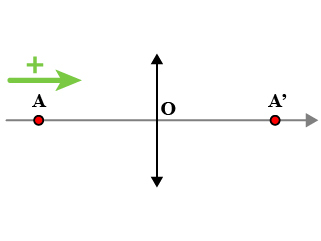
\includegraphics[max size={\textwidth}{0.9\textheight}, center, keepaspectratio]{QCM/Physique/UTC-002/lentille.jpg}
\end{minipage}
}

%%% QUESTION %%% 
\vspace*{\stretch{1}}
%%% ANSWER %%% 
\color{white}

% Correct answer boxes
\begin{tikzpicture}[remember picture, overlay]
    \node [align=left, opacity=1] at ([xshift = 4.75 cm, yshift = -9.85 cm]current page.north west) {
                \color{white}
                \normalsize
                \textsf{\textit{Réponses}}
            };
    \node [align=left, opacity=1] at ([xshift = 7.75 cm, yshift = -9.85 cm]current page.north west) {
                \color{white}
                $1:\boxtimes\qquad2:\square\qquad3:\square\qquad4:\square\qquad$\\
                \color{white}
                $5:\square\qquad6:\square\qquad$
            };
\end{tikzpicture}

% Explanations
\RaggedRight
\vspace{0.09\cardheight}

Principe d'inertie : Dans un référentiel galiléen, si un système assimilé à un point matériel n'est soumis à aucune force – système isolé – ou s'il est soumis à un ensemble de forces de résultante nulle ($\Sigma\vec{F}_{ext}=\vec{0}$) – système pseudo-isolé – alors il est immobile ou animé d'un mouvement rectiligne uniforme.

Dans cette question, il s'agit de faire la distinction entre mouvement uniforme (la norme de la vitesse est constante, on ne sait rien de la trajectoire) et mouvement rectiligne uniforme ou mouvement circulaire uniforme (norme de la vitesse constante et trajectoire fixée).

%%% ANSWER %%% 
\vspace*{\stretch{1}}
\end{flashcard}

% Test flashcard n°2b
\begin{flashcard}[]{
%%% QUESTION %%% 
\color{black}
\vspace{0.12\cardheight}
\RaggedRight
% Topic
\begin{minipage}[t]{0.6\linewidth}
Étant donné le sens de propagation de la lumière choisi et indiqué sur le schéma, si $A$ est la position de l'objet, $A'$ celle de l'image et $O$ le centre de la lentille convergente, alors :
% Choices
\begin{enumerate}
    \item $\overline{OA}$ est positif et $\overline{OA'}$ est négatif.
    \item $\overline{OA}$ est négatif et $\overline{OA'}$ est positif.
    \item $\overline{OA}$ et $\overline{OA'}$ sont négatifs.
    \item $\overline{OA}$ et $\overline{OA'}$ sont positifs.
\end{enumerate}
\end{minipage}% 
\hfill
% Image
\begin{minipage}[t]{0.3\linewidth}
    \strut\vspace*{-\baselineskip}\newline
    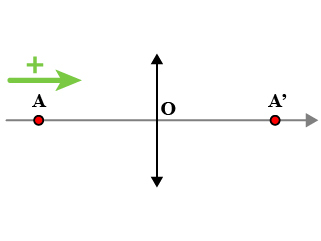
\includegraphics[max size={\textwidth}{0.9\textheight}, center, keepaspectratio]{QCM/Physique/UTC-002/lentille.jpg}
\end{minipage}
}

%%% QUESTION %%% 
\vspace*{\stretch{1}}
%%% ANSWER %%% 
\color{white}

% Correct answer boxes
\begin{tikzpicture}[remember picture, overlay]
    \node [align=left, opacity=1] at ([xshift = 14.75 cm, yshift = -17.95 cm]current page.north west) {
                \color{white}
                \normalsize
                \textsf{\textit{Réponses}}
            };
    \node [align=left, opacity=1] at ([xshift = 17.75 cm, yshift = -17.95 cm]current page.north west) {
                \color{white}
                $1:\boxtimes\qquad2:\square\qquad3:\square\qquad4:\square\qquad$\\
                \color{white}
                $5:\square\qquad6:\square\qquad$
            };
\end{tikzpicture}

% Explanations
\RaggedRight
\vspace{0.09\cardheight}

Principe d'inertie : Dans un référentiel galiléen, si un système assimilé à un point matériel n'est soumis à aucune force – système isolé – ou s'il est soumis à un ensemble de forces de résultante nulle ($\Sigma\vec{F}_{ext}=\vec{0}$) – système pseudo-isolé – alors il est immobile ou animé d'un mouvement rectiligne uniforme.

Dans cette question, il s'agit de faire la distinction entre mouvement uniforme (la norme de la vitesse est constante, on ne sait rien de la trajectoire) et mouvement rectiligne uniforme ou mouvement circulaire uniforme (norme de la vitesse constante et trajectoire fixée).

%%% ANSWER %%% 
\vspace*{\stretch{1}}
\end{flashcard}
% Test flashcard n°2c

\begin{flashcard}[]{
%%% QUESTION %%% 
\color{black}
\vspace{0.12\cardheight}
\RaggedRight
% Topic
\begin{minipage}[t]{0.6\linewidth}
Étant donné le sens de propagation de la lumière choisi et indiqué sur le schéma, si $A$ est la position de l'objet, $A'$ celle de l'image et $O$ le centre de la lentille convergente, alors :
% Choices
\begin{enumerate}
    \item $\overline{OA}$ est positif et $\overline{OA'}$ est négatif.
    \item $\overline{OA}$ est négatif et $\overline{OA'}$ est positif.
    \item $\overline{OA}$ et $\overline{OA'}$ sont négatifs.
    \item $\overline{OA}$ et $\overline{OA'}$ sont positifs.
\end{enumerate}
\end{minipage}% 
\hfill
% Image
\begin{minipage}[t]{0.3\linewidth}
    \strut\vspace*{-\baselineskip}\newline
    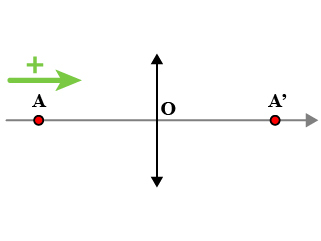
\includegraphics[max size={\textwidth}{0.9\textheight}, center, keepaspectratio]{QCM/Physique/UTC-002/lentille.jpg}
\end{minipage}
}

%%% QUESTION %%% 
\vspace*{\stretch{1}}
%%% ANSWER %%% 
\color{white}

% Correct answer boxes
\begin{tikzpicture}[remember picture, overlay]
    \node [align=left, opacity=1] at ([xshift = 4.75 cm, yshift = -17.95 cm]current page.north west) {
                \color{white}
                \normalsize
                \textsf{\textit{Réponses}}
            };
    \node [align=left, opacity=1] at ([xshift = 7.75 cm, yshift = -17.95 cm]current page.north west) {
                \color{white}
                $1:\boxtimes\qquad2:\square\qquad3:\square\qquad4:\square\qquad$\\
                \color{white}
                $5:\square\qquad6:\square\qquad$
            };
\end{tikzpicture}

% Explanations
\RaggedRight
\vspace{0.09\cardheight}

Principe d'inertie : Dans un référentiel galiléen, si un système assimilé à un point matériel n'est soumis à aucune force – système isolé – ou s'il est soumis à un ensemble de forces de résultante nulle ($\Sigma\vec{F}_{ext}=\vec{0}$) – système pseudo-isolé – alors il est immobile ou animé d'un mouvement rectiligne uniforme.

Dans cette question, il s'agit de faire la distinction entre mouvement uniforme (la norme de la vitesse est constante, on ne sait rien de la trajectoire) et mouvement rectiligne uniforme ou mouvement circulaire uniforme (norme de la vitesse constante et trajectoire fixée).

%%% ANSWER %%% 
\vspace*{\stretch{1}}
\end{flashcard}

% New set of 6 flashcards
\setkeys{One}{
    complexityLevel = {Changement de langage},
    subject = {Physique},
    theme = {Optique géométrique},
    qrcode = {qrcode}
}
\cardbackground{1}
% Test flashcard n°2d

\begin{flashcard}[]{
%%% QUESTION %%% 
\color{black}
\vspace{0.12\cardheight}
\RaggedRight
% Topic
\begin{minipage}[t]{0.6\linewidth}
Étant donné le sens de propagation de la lumière choisi et indiqué sur le schéma, si $A$ est la position de l'objet, $A'$ celle de l'image et $O$ le centre de la lentille convergente, alors :
% Choices
\begin{enumerate}
    \item $\overline{OA}$ est positif et $\overline{OA'}$ est négatif.
    \item $\overline{OA}$ est négatif et $\overline{OA'}$ est positif.
    \item $\overline{OA}$ et $\overline{OA'}$ sont négatifs.
    \item $\overline{OA}$ et $\overline{OA'}$ sont positifs.
\end{enumerate}
\end{minipage}% 
\hfill
% Image
\begin{minipage}[t]{0.3\linewidth}
    \strut\vspace*{-\baselineskip}\newline
    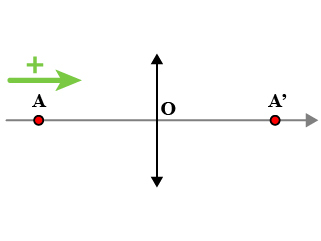
\includegraphics[max size={\textwidth}{0.9\textheight}, center, keepaspectratio]{QCM/Physique/UTC-002/lentille.jpg}
\end{minipage}
}

%%% QUESTION %%% 
\vspace*{\stretch{1}}
%%% ANSWER %%% 
\color{white}

% Correct answer boxes
\begin{tikzpicture}[remember picture, overlay]
    \node [align=left, opacity=1] at ([xshift = 14.75 cm, yshift = -1.75 cm]current page.north west) {
                \color{white}
                \normalsize
                \textsf{\textit{Réponses}}
            };
    \node [align=left, opacity=1] at ([xshift = 17.75 cm, yshift = -1.75 cm]current page.north west) {
                \color{white}
                $1:\boxtimes\qquad2:\square\qquad3:\square\qquad4:\square\qquad$\\
                \color{white}
                $5:\square\qquad6:\square\qquad$
            };
\end{tikzpicture}

% Explanations
\vspace{0.09\cardheight}
\RaggedRight

Principe d'inertie : Dans un référentiel galiléen, si un système assimilé à un point matériel n'est soumis à aucune force – système isolé – ou s'il est soumis à un ensemble de forces de résultante nulle ($\Sigma\vec{F}_{ext}=\vec{0}$) – système pseudo-isolé – alors il est immobile ou animé d'un mouvement rectiligne uniforme.

Dans cette question, il s'agit de faire la distinction entre mouvement uniforme (la norme de la vitesse est constante, on ne sait rien de la trajectoire) et mouvement rectiligne uniforme ou mouvement circulaire uniforme (norme de la vitesse constante et trajectoire fixée).

%%% ANSWER %%% 
\vspace*{\stretch{1}}
\end{flashcard}

\end{document}